\documentclass[12pt]{article}

% --- Packages ---
\usepackage[utf8]{inputenc}
\usepackage[T1]{fontenc}
\usepackage[french]{babel}
\usepackage{amsmath, amssymb}
\usepackage{geometry}
\usepackage{tikz}
\usepackage[most]{tcolorbox}
\usepackage{lmodern}
\usepackage{pgfplots}
\pgfplotsset{compat=1.18}
\usepackage{mdframed}
\usepackage{bm}
\usepackage{xcolor}
\usepackage{sectsty}
\usetikzlibrary{calc}

\usepackage[utf8]{inputenc}
\usepackage[T1]{fontenc}
\usepackage[dvipsnames]{xcolor}
\usepackage{tkz-tab}
\usepackage{multido}
% --- Page ---
\geometry{margin=2cm}

% Footer
\usepackage{fancyhdr}
\pagestyle{fancy}
\cfoot{\thepage}
\rfoot{\textit{G.M.}}
\renewcommand{\headrulewidth}{0pt}
\renewcommand{\footrulewidth}{0pt}

% Pour les normes : 
\newcommand*{\norme}[1]{\left\lVert\overrightarrow{#1}\right\rVert}

% Pour le det
\newcommand*{\Det}[4]{% 
  \ensuremath{
    \begin{vmatrix} 
      #1 & #2 \\
      #3 & #4 
    \end{vmatrix}}}

% Pour les coordonnées de vecteurs :
\newcommand*{\Coord}[2]{% 
  \ensuremath{
    \begin{pmatrix} 
      #1\\ 
      #2 
    \end{pmatrix}}}

% % Pour les coordonnées de points :
% \newcommand*{\Coord}[3]{% 
%   \ensuremath{#1\,
%     \begin{pmatrix}
%       #2\\ 
%       #3 
%     \end{pmatrix}}}

\usetikzlibrary{shapes.misc}

\tikzset{cross/.style={cross out, draw=black, minimum size=2*(#1-\pgflinewidth), inner sep=0pt, outer sep=0pt},
%default radius will be 1pt. 
cross/.default={4pt}}

% mettre dans le préambule, après \usepackage{xcolor}
\usepackage{sectsty} % gère facilement la couleur des titres
\setlength{\parindent}{0pt}

\sectionfont{\color{red}\Large\bfseries}     % pour \section*
% \subsectionfont{\color{red}\normalsize\bfseries} % pour \subsection*
\subsectionfont{\color{red}\large\bfseries\hspace{1cm}}

\begin{document}

\begin{center}
    {\LARGE \textbf{Droites du plan}}\\[2mm]
    {\large Classe de 2nde}
\end{center}

% ============================
%   PARTIE 1 : Vecteur directeur et équation cartésienne d'une droite
% ============================

\section*{\textcolor{red}{Partie 1 : Vecteur directeur et équation cartésienne d'une droite}}

% ========================================================
%             1) Vecteur directeur
% ========================================================
\subsection*{\textcolor{red}{1) Vecteur directeur}}

\vspace{5pt}

\begin{mdframed}[
    linewidth=1pt,
    roundcorner=5pt,
    linecolor=ForestGreen,
    innertopmargin=10pt,
    innerbottommargin=10pt
]
{\color{ForestGreen}
\textbf{\underline{Définition :}}}

\vspace{0pt}
\begin{minipage}[t]{.55\textwidth}%
    \vspace{0pt}
    $d$ est une droite du plan.

    On appelle \textbf{vecteur directeur} de $d$ tout vecteur non nul $\overrightarrow{u}$
    qui possède la même \textbf{direction} que la droite $d$.
\end{minipage}%
\hfill
\begin{minipage}[t]{.35\textwidth}%
    \vspace{-20pt}
    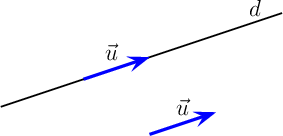
\includegraphics[width=0.8\textwidth]{4.png}
\end{minipage}%

\end{mdframed}

\vspace{10pt}
\textbf{\underline{Méthode :} Déterminer graphiquement un vecteur directeur d'une droite.}

\begin{minipage}[t]{.5\textwidth}%
    \vspace{0pt}
    On cherche des vecteurs directeurs pour $d_1$, $d_2$, $d_3$ et $d_4$.

    \vspace{5pt}
    \hspace{1cm}\textbullet $d_1$ :

    On cherche un vecteur qui possède la même direction que $d_1$ et on calcule 
    ses coordonnées.

    Par exemple : 
    \begin{center}
        $\overrightarrow{a}\Coord{\ \ \ \ \ \ }{\ \ \ }$ \hspace{0.2cm} ou \hspace{0.2cm}
        $\overrightarrow{b}\Coord{\ \ \ \ \ \ }{\ \ \ }$ \hspace{0.2cm} ou \hspace{0.2cm}
        $\overrightarrow{c}\Coord{\ \ \ \ \ \ }{\ \ \ }$
        
        \vspace{10pt}
        conviennent.
    \end{center}

    \vspace{5pt}
    \hspace{1cm}\textbullet $d_2$ :

    \vspace{1cm}

\end{minipage}%
\hfill
\begin{minipage}[t]{.45\textwidth}%
    \vspace{0pt}
    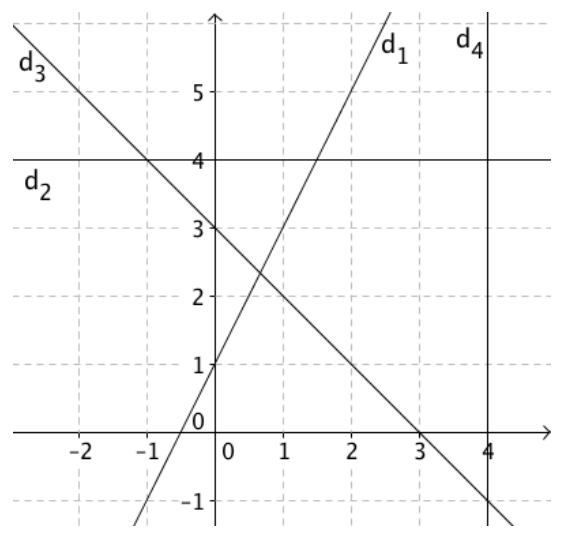
\includegraphics[width=0.9\textwidth]{methode1.png}
\end{minipage}%

\vspace{5pt}
\hspace{1cm}\textbullet $d_3$ : \hspace{5cm} \hspace{1cm}\textbullet $d_4$ :

\vspace{0.5cm}


% ========================================================
%             2) Équation cartésienne d'une droite
% ========================================================
\subsection*{\textcolor{red}{2) Équation cartésienne d'une droite}}

\vspace{5pt}

\begin{mdframed}[
    linewidth=1pt,
    roundcorner=5pt,
    linecolor=ForestGreen,
    innertopmargin=10pt,
    innerbottommargin=10pt
]
{\color{ForestGreen}
\textbf{\underline{Définition :}}}

\vspace{5pt}
Toute droite admet une équation de la forme 
\[
    \bm{ax + by + c = 0} \quad \text{avec} \quad (a;b) \neq (0;0)
\]

\vspace{5pt}
Cette équation est appelée \textbf{équation cartésienne} de la droite.

\end{mdframed}

\begin{mdframed}[
    linewidth=1pt,
    roundcorner=5pt,
    linecolor=Red,
    innertopmargin=10pt,
    innerbottommargin=5pt
]
{\color{red}
\textbf{\underline{Propriété :}}

\vspace{5pt}
 Le vecteur $\overrightarrow{u}\Coord{-b}{a}$ est un vecteur directeur de la droite 
 d’équation cartésienne $ax + by + c = 0$.
}
\end{mdframed}

\begin{mdframed}[
    linewidth=1pt,
    roundcorner=5pt,
    linecolor=RoyalBlue,
    innertopmargin=10pt,
    innerbottommargin=10pt
]
{\color{RoyalBlue}
\textbf{\underline{Démonstration:}}}

\vspace{5pt}
Soit $A\Coord{x_0}{y_0}$ un point de la droite $d$ et $\overrightarrow{u}
\Coord{\alpha}{\beta}$ un vecteur directeur de $d$.

Un point $M\Coord{x}{y}$ appartient à la droite $d$ si et seulement si les 
vecteurs $\overrightarrow{AM}\Coord{x-x_0}{y-y_0}$ et $\overrightarrow{u}$
sont colinéaires, soit $det(\overrightarrow{AM};\overrightarrow{u}) = 0$ soit encore 
$\Det{x-x_0}{\alpha}{y-y_0}{\beta} = 0$.

\vspace{5pt}
Donc : $\beta(x-x_0) - \alpha(y-y_0) = 0$

$\beta x - \beta x_0 - \alpha y + \alpha y_0 = 0$

$\beta x - \alpha y  + \alpha y_0 - \beta x_0 = 0$

\vspace{5pt}
Cette équation peut s'écrire : $ax + by + c = 0$ avec $a = \beta$ et $b = -\alpha$
et $c = \alpha y_0 - \beta x_0$.

Les coordonnées de $\overrightarrow{u}$ sont donc $\Coord{\alpha}{\beta} 
= \Coord{-b}{a}$.

\end{mdframed}

\vspace{10pt}
{\color{RedOrange}\textbf{\underline{Méthode :} Déterminer un vecteur directeur d'une droite à partir
de son équation cartésienne.}}

\vspace{5pt}
\hspace{1cm}\textbullet$d_1$ a pour équation cartésienne $4x - 5y - 1 = 0$.

\vspace{5pt}
On commence par déterminer $a$ et $b$ :

\vspace{10pt}
\hspace{1cm}$a = $ \hspace{2cm} et $b = $

\vspace{10pt}
Puis on détermine le vecteur directeur de $d_1$ : $\overrightarrow{u}\Coord{-b}{a} 
\quad = \quad \overrightarrow{u}\Coord{\ \ \ \ \ \ }{\ \ \ \ \ \ }$

\vspace{10pt}
\hspace{1cm}\textbullet$d_2$ a pour équation cartésienne $-3x + 4y - 2 = 0$.

\vspace{5pt}
Un vecteur directeur est : 

\vspace{2cm}

{\color{RedOrange}\textbf{\underline{Méthode :} Déterminer une équation cartésienne de 
droite à partir d'un point et d'un vecteur directeur.}}

\vspace{5pt}
\hspace{1cm}a) Déterminer une équation cartésienne de la droite $d$ passant par 
$A\Coord{3}{1}$ et de vecteur directeur $\overrightarrow{u}\Coord{-1}{5}$.

\vspace{5pt}
$\overrightarrow{u}$ étant vecteur directeur de $d$, on a 
$\Coord{\ \ \ \ \ \ }{\ \ \ \ \ \ } = \Coord{\ \ \ \ \ \ }{\ \ \ \ \ \ }$

Soit $a = $ \hspace{1cm} et $b = $

\vspace{5pt}
L'équation de $d$ est donc : 

\vspace{5pt}
Il nous faut maintenant trouver $c$.

\vspace{5pt}
Pour cela, il suffit de substituer les coordonnées de $A$ dans l'équation, car 
\textbf{$\bm{A}$ appartient à cette droite et vérifie donc son équation}.

\vspace{0.5cm}
{\color{black!30}\dotfill}

\vspace{0.5cm}
{\color{black!30}\dotfill}

\vspace{20pt}


\underline{Remarque :}

Une autre méthode consiste à utiliser le déterminant :

\vspace{5pt}
On choisit un point $M\Coord{x}{y}$ appartenant à la droite. Alors forcément, le vecteur 
$\overrightarrow{AM}$ et le vecteur $\overrightarrow{u}$ seront colinéaires. 
On aura donc $det(\overrightarrow{AM};\overrightarrow{u}) = 0$ :

\vspace{0.5cm}
{\color{black!30}\dotfill}

\vspace{0.5cm}
{\color{black!30}\dotfill}

\vspace{0.5cm}
{\color{black!30}\dotfill}

\vspace{0.5cm}
{\color{black!30}\dotfill}

\vspace{20pt}

\begin{mdframed}[
    linewidth=1pt,
    roundcorner=5pt,
    linecolor=RoyalBlue,
    innertopmargin=10pt,
    innerbottommargin=10pt
]
{\color{RoyalBlue}
\textbf{\underline{Exercice d'application n°1:} Déterminer une équation cartésienne d'une
droite.}}

\vspace{5pt}
Déterminer une équation cartésienne de la droite passant par le point $A\Coord{-1}{2}$ et de 
vecteur directeur $\overrightarrow{u}\Coord{-3}{1}$.

\vspace{0.5cm}
{\color{black!30}\dotfill}

\vspace{0.5cm}
{\color{black!30}\dotfill}

\vspace{0.5cm}
{\color{black!30}\dotfill}

\vspace{0.5cm}
{\color{black!30}\dotfill}

\vspace{0.5cm}
{\color{black!30}\dotfill}

\vspace{0.5cm}
{\color{black!30}\dotfill}

\vspace{20pt}

\newpage
{\color{RoyalBlue}
\textbf{\underline{Exercice d'application n°2:} Déterminer une équation cartésienne d'une
droite.}}

\vspace{5pt}
\begin{minipage}[t]{.45\textwidth}%
    \vspace{5pt}
    Pour chacune de ces droites, donner un vecteur directeur, un point et une équation 
    cartésienne.

    \vspace{0.5cm}
    {\color{black!30}\dotfill}
    
    \vspace{0.5cm}
    {\color{black!30}\dotfill}
    
    \vspace{0.5cm}
    {\color{black!30}\dotfill}
    
    \vspace{0.5cm}
    {\color{black!30}\dotfill}
    
    \vspace{0.5cm}
    {\color{black!30}\dotfill}
    
\end{minipage}%
\hfill
\begin{minipage}[t]{.45\textwidth}%
    \vspace{0pt}
    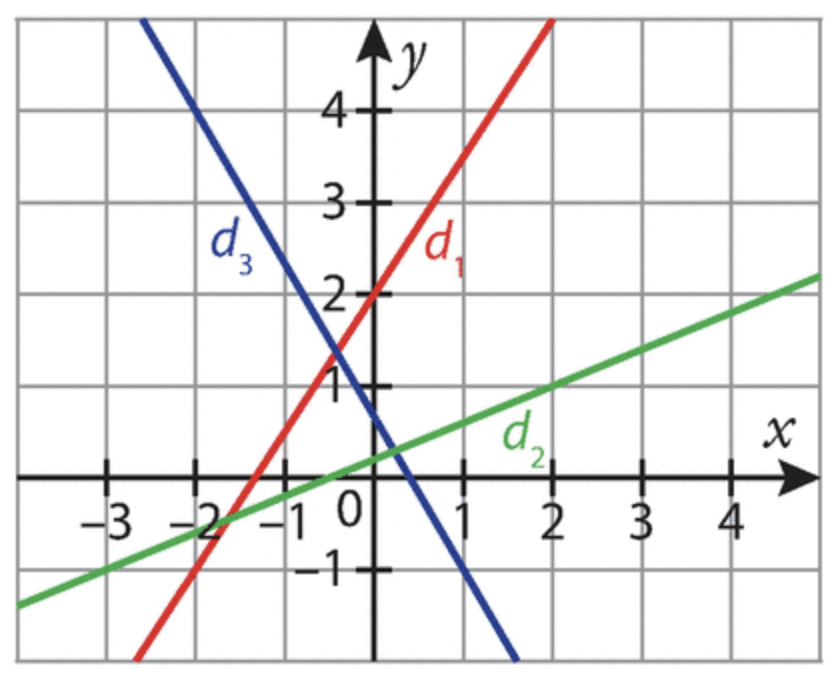
\includegraphics[width=1\textwidth]{exer2.png}
\end{minipage}%

\vspace{13pt}
\vspace{0.5cm}
{\color{black!30}\dotfill}

\vspace{0.5cm}
{\color{black!30}\dotfill}

\vspace{0.5cm}
{\color{black!30}\dotfill}

\vspace{0.5cm}
{\color{black!30}\dotfill}

\vspace{0.5cm}
{\color{black!30}\dotfill}

\vspace{0.5cm}
{\color{black!30}\dotfill}

\vspace{0.5cm}
{\color{black!30}\dotfill}

\vspace{0.5cm}
{\color{black!30}\dotfill}


\vspace{20pt}


\end{mdframed}

\vspace{10pt}
{\color{RedOrange}\textbf{\underline{Méthode :} Tracer une droite à partir de l'équation
cartésienne.}}

\vspace{5pt}
\textbf{Tracer la droite $\bm{(d)}$ d'équation cartésienne $\bm{3x + 2y - 5 = 0}$.}

\vspace{5pt}
Pour tracer une droite il nous suffit de connaître \textbf{un point} de la droite et un \textbf{vecteur directeur}.

\vspace{10pt}
\textbullet On fixe une abscisse ou une ordonnée au hasard et on calcul la deuxième
coordonnée : 

\vspace{0.5cm}
{\color{black!30}\dotfill}

\vspace{0.5cm}
{\color{black!30}\dotfill}

\vspace{0.5cm}
{\color{black!30}\dotfill}

\vspace{20pt}

Puis on calcul un vecteur directeur et on trace la droite à l'aide du point et du vecteur : 

\begin{minipage}[t]{.45\textwidth}%
    \vspace{0pt}
    \vspace{0.5cm}
    {\color{black!30}\dotfill}
    
    \vspace{0.5cm}
    {\color{black!30}\dotfill}
    
    \vspace{0.5cm}
    {\color{black!30}\dotfill}
    
    \vspace{0.5cm}
    {\color{black!30}\dotfill}
    
    \vspace{0.5cm}
    {\color{black!30}\dotfill}

    \vspace{0.5cm}
    {\color{black!30}\dotfill}
    
    \vspace{0.5cm}
    {\color{black!30}\dotfill}
    
    \vspace{0.5cm}
    {\color{black!30}\dotfill}
    
    
    \vspace{20pt}
\end{minipage}%
\hfill
\begin{minipage}[t]{.45\textwidth}%
    \vspace{0pt}
    \begin{tikzpicture}
    \begin{axis}[
        width=9cm,
        height=9cm,
        axis lines=center,
        grid=both,
        grid style={line width=.1pt, draw=gray},
        xmin=-4, xmax=4,
        ymin=-2, ymax=6,
        samples=200,
        xlabel={$x$},
        ylabel={$y$},
        legend pos=north west,
        legend cell align=left
    ]
    \end{axis}
    \end{tikzpicture}
\end{minipage}%

\begin{mdframed}[
    linewidth=1pt,
    roundcorner=5pt,
    linecolor=RoyalBlue,
    innertopmargin=10pt,
    innerbottommargin=10pt
]
{\color{RoyalBlue}
\textbf{\underline{Exercice d'application n°3:} Tracer une droite dans un repère orthonormé.}}

\vspace{5pt}
Tracer la droite $(d_1)$ d'équation cartésienne : $-x + 2y + 4 = 0$

\begin{minipage}[t]{.45\textwidth}%
    \vspace{0pt}
    \vspace{0.5cm}
    {\color{black!30}\dotfill}
    
    \vspace{0.5cm}
    {\color{black!30}\dotfill}
    
    \vspace{0.5cm}
    {\color{black!30}\dotfill}
    
    \vspace{0.5cm}
    {\color{black!30}\dotfill}
    
    \vspace{0.5cm}
    {\color{black!30}\dotfill}

    \vspace{0.5cm}
    {\color{black!30}\dotfill}
    
    \vspace{20pt}
\end{minipage}%
\hfill
\begin{minipage}[t]{.45\textwidth}%
    \vspace{0pt}
    \begin{tikzpicture}
    \begin{axis}[
        width=9cm,
        height=8cm,
        axis lines=center,
        grid=both,
        grid style={line width=.1pt, draw=gray},
        xmin=-4, xmax=4,
        ymin=-4, ymax=2,
        samples=200,
        xlabel={$x$},
        ylabel={$y$},
        legend pos=north west,
        legend cell align=left
    ]
    \end{axis}
    \end{tikzpicture}
\end{minipage}%

\end{mdframed}

% ========================================================
%             3) Positions relatives de deux droites
% ========================================================
\hspace{1cm}\subsection*{\textcolor{red}{3) Positions relatives de deux droites}}

\vspace{5pt}
\begin{mdframed}[
    linewidth=1pt,
    roundcorner=5pt,
    linecolor=Red,
    innertopmargin=10pt,
    innerbottommargin=10pt
]
{\color{red}
\textbf{\underline{Propriété :}}

\vspace{5pt}
Dire que deux droites sont \textbf{parallèles} équivaut à dire que leurs \textbf{vecteurs directeurs} 
sont \textbf{colinéaires}.
}
\end{mdframed}

\newpage
{\color{RedOrange}\textbf{\underline{Méthode :} Déterminer la position relative de deux droites.}}

\vspace{5pt}
\textbf{Démontrer que les droites $(d_1)$ et $(d_2)$ d'équations cartésiennes respectives $6x-10y-5 = 0$ et 
$-9x+15y = 0$ sont parallèles.}

\vspace{10pt}
Il suffit de trouver des vecteurs directeurs et de vérifier qu'ils sont bien colinéaires.

\vspace{0.5cm}
{\color{black!30}\dotfill}

\vspace{0.5cm}
{\color{black!30}\dotfill}

\vspace{0.5cm}
{\color{black!30}\dotfill}

\vspace{0.5cm}
{\color{black!30}\dotfill}

\vspace{0.5cm}
{\color{black!30}\dotfill}

\vspace{0.5cm}
{\color{black!30}\dotfill}

\vspace{0.5cm}
{\color{black!30}\dotfill}

\vspace{20pt}

\begin{mdframed}[
    linewidth=1pt,
    roundcorner=5pt,
    linecolor=RoyalBlue,
    innertopmargin=10pt,
    innerbottommargin=10pt
]
{\color{RoyalBlue}
\textbf{\underline{Exercice d'application n°4:} Déterminer les positions relatives de deux droites.}}

\vspace{5pt}
Déterminer les positions relatives des droites $(d_1)$ et $(d_2)$ d'équations cartésiennes 
respectives $\dfrac{7}{3}x - y +2=0$ et 
$7x - 3y +9 = 0$.

\vspace{0.5cm}
{\color{black!30}\dotfill}

\vspace{0.5cm}
{\color{black!30}\dotfill}

\vspace{0.5cm}
{\color{black!30}\dotfill}

\vspace{0.5cm}
{\color{black!30}\dotfill}

\vspace{0.5cm}
{\color{black!30}\dotfill}

\vspace{0.5cm}
{\color{black!30}\dotfill}
\vspace{0.5cm}
{\color{black!30}\dotfill}

\vspace{0.5cm}
{\color{black!30}\dotfill}

\vspace{0.5cm}
{\color{black!30}\dotfill}

\vspace{0.5cm}
{\color{black!30}\dotfill}

\vspace{20pt}

\end{mdframed}


\newpage

% ============================
%   PARTIE 2 : Équation réduite et pente d'une droite
% ============================

\section*{\textcolor{red}{Partie 2 : Équation réduite et pente d'une droite}}

% ========================================================
%             1) Équation réduite
% ========================================================
\vspace{5pt}
\subsection*{\textcolor{red}{1) Équation réduite}}

\vspace{5pt}
\underline{\textbf{Exemple :}}

\vspace{5pt}
Soit $(d)$ une droite d'équation cartésienne $4x+y-6 = 0$.
Isolons alors $y$ : 

\vspace{0.5cm}
{\color{black!30}\dotfill}

\vspace{0.5cm}
{\color{black!30}\dotfill}

\vspace{0.5cm}
{\color{black!30}\dotfill}

\vspace{20pt}
Cette équation est appelée \textbf{{\color{red}équation réduite}} de la droite $(d)$.

\vspace{10pt}

\begin{mdframed}[
    linewidth=1pt,
    roundcorner=5pt,
    linecolor=Red,
    innertopmargin=10pt,
    innerbottommargin=10pt
]
{\color{red}
\textbf{\underline{Propriété :}}

\vspace{5pt}
Soit $(d)$ une droite.

\begin{minipage}[t]{.45\textwidth}%
    \vspace{0pt}
    \begin{itemize}
        \item Si $(d)$ est parallèle à l'axe des ordonnées, son équation est de la forme : $x = n$.
        \vspace{40pt}
        \item Si $(d)$ est parallèle à l'axe des abscisses, son équation est de la forme : $y = b$.
        \vspace{40pt}
        \item Sinon alors son équation est de la forme $y = ax + b$. C'est \textbf{l'équation réduite de la 
        droite $(d)$.}
    \end{itemize}
\end{minipage}%
\hfill
\begin{minipage}[t]{.5\textwidth}%
    \vspace{-40pt}
    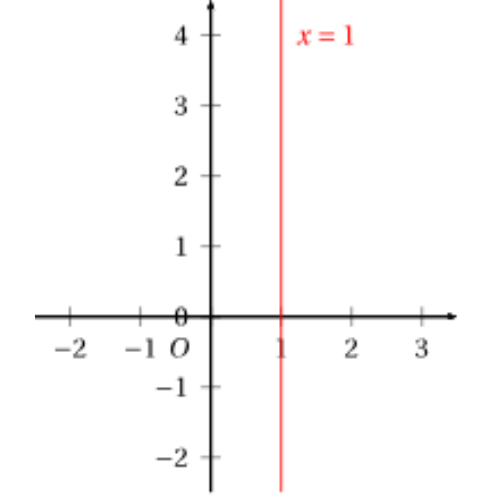
\includegraphics[width=0.5\textwidth]{droite verticale.png}

    \vspace{-40pt}
    \hspace{4cm}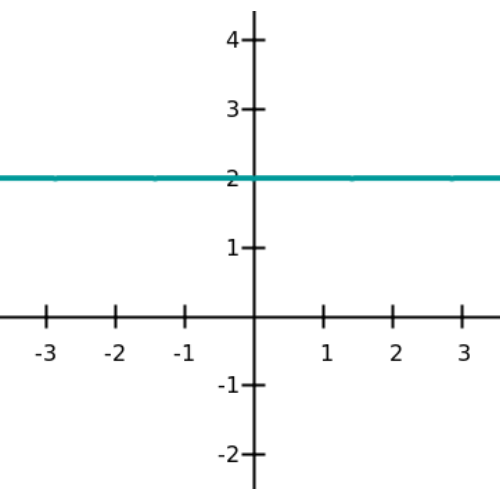
\includegraphics[width=0.5\textwidth]{droite horiz.png}

    \vspace{-30pt}
    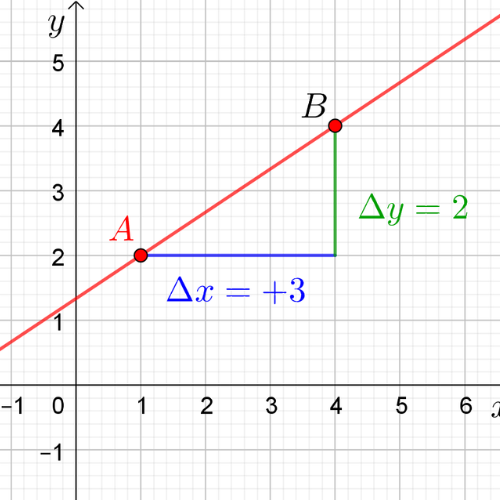
\includegraphics[width=0.5\textwidth]{droite.png}
\end{minipage}%

}
\end{mdframed}

\begin{mdframed}[
    linewidth=1pt,
    roundcorner=5pt,
    linecolor=RoyalBlue,
    innertopmargin=10pt,
    innerbottommargin=10pt
]
{\color{RoyalBlue}
\textbf{\underline{Exercice d'application n°5:} Passer d'une équation cartésienne à une équation réduite 
et inversement.}}

\vspace{5pt}
\hspace{1cm}a) Soit la droite $(d)$ d’équation cartésienne $6x + 3y - 5 = 0$. 

\hspace{1.5cm}Déterminer l’équation réduite de $(d)$.

\vspace{5pt}
\hspace{1cm}b) Soit la droite $(d')$ d’équation réduite $y = 6x - 5$.

\hspace{1.5cm}Déterminer une équation catésienne de $(d')$.

\vspace{0.5cm}
{\color{black!30}\dotfill}

\vspace{0.5cm}
{\color{black!30}\dotfill}

\vspace{0.5cm}
{\color{black!30}\dotfill}

\vspace{0.5cm}
{\color{black!30}\dotfill}

\vspace{20pt}

{\color{RoyalBlue}
\textbf{\underline{Exercice d'application n°6:} Représenter graphiquement une droite d’équation réduite 
donnée.}}

\vspace{5pt}
\begin{minipage}[t]{.45\textwidth}%
    \vspace{0pt}
    Dans le repère, tracer les droites $(d_1)$, $(d_2)$ et $(d_3)$ d’équations respectives :

    $y = 2x + 3$, $y = 4$ et $x = 3$.

    \vspace{0.5cm}
    {\color{black!30}\dotfill}
    
    \vspace{0.5cm}
    {\color{black!30}\dotfill}
    
    \vspace{0.5cm}
    {\color{black!30}\dotfill}
    
    \vspace{0.5cm}
    {\color{black!30}\dotfill}

    \vspace{0.5cm}
    {\color{black!30}\dotfill}
    
    \vspace{0.5cm}
    {\color{black!30}\dotfill}
    
    \vspace{20pt}
\end{minipage}%
\hfill
\begin{minipage}[t]{.5\textwidth}%
    \vspace{-20pt}
    \begin{tikzpicture}
    \begin{axis}[
        width=9cm,
        height=10cm,
        axis lines=center,
        grid=both,
        grid style={line width=.1pt, draw=gray},
        xmin=-3, xmax=4,
        ymin=-1, ymax=7,
        samples=200,
        xlabel={$x$},
        ylabel={$y$},
        legend pos=north west,
        legend cell align=left
    ]
    \end{axis}
    \end{tikzpicture}
\end{minipage}%

\end{mdframed}

% ========================================================
%             2) Positions relatives et équations réduites
% ========================================================
\vspace{5pt}
\subsection*{\textcolor{red}{2) Positions relatives et équations réduites}}

\begin{mdframed}[
    linewidth=1pt,
    roundcorner=5pt,
    linecolor=Red,
    innertopmargin=10pt,
    innerbottommargin=10pt
]
{\color{red}
\textbf{\underline{Propriété :}}

\vspace{5pt}
Soient deux droites d'équations \textbf{\underline{réduites}} $y = ax + b$ et $y = a'x + b'$.

\vspace{5pt}
Dire que les droites sont parallèles revient à dire que leurs pentes sont égales : $a = a'$.
}
\end{mdframed}

\underline{Remarque :} Lorsque les pentes sont différentes, les droites sont \textbf{sécantes}.

\vspace{5pt}
\begin{mdframed}[
    linewidth=1pt,
    roundcorner=5pt,
    linecolor=RoyalBlue,
    innertopmargin=10pt,
    innerbottommargin=10pt
]
{\color{RoyalBlue}
\textbf{\underline{Exercice d'application n°7:} Déterminer la position relative de deux droites à partir 
de leurs équations réduites.}}

\vspace{5pt}
Dans chaque cas, déterminer la position relative des deux droites :

\vspace{5pt}
\hspace{1cm}a) $(d_1) : y = -2x - 5$ et $(d_2) : y = -2x + 4$

\vspace{5pt}
\hspace{1cm}b) $(d_3) : y = 2x + 1$ et $(d_4) : y = -3x + 8$

\vspace{5pt}
\hspace{1cm}c) $(d_5) : y = -x + 7$ et $(d_6) : y = 3$

\vspace{5pt}
\hspace{1cm}d) $(d_7) : x = 1$ et $(d_8) : x = -8$

\vspace{0.5cm}
{\color{black!30}\dotfill}

\vspace{0.5cm}
{\color{black!30}\dotfill}

\vspace{0.5cm}
{\color{black!30}\dotfill}

\vspace{0.5cm}
{\color{black!30}\dotfill}

\vspace{0.5cm}
{\color{black!30}\dotfill}

\vspace{20pt}

\end{mdframed}

\vspace{20pt}

% ========================================================
%             PARTIE 3 : Projeté orthogonal d'un point sur une droite
% ========================================================

\section*{\textcolor{red}{Partie 3 : Projeté orthogonal d'un point sur une droite}}

\vspace{5pt}
\begin{mdframed}[
    linewidth=1pt,
    roundcorner=5pt,
    linecolor=ForestGreen,
    innertopmargin=10pt,
    innerbottommargin=10pt
]
{\color{ForestGreen}
\textbf{\underline{Définition :}}}

\vspace{15pt}
Soit une droite $(d)$ et un point $M$.

\vspace{5pt}
\begin{minipage}[t]{.45\textwidth}%
    \vspace{0pt}
    Le \textbf{projeté orthonal} du point $M$ sur la droite $(d)$ est le point d'intersection $H$ de la droite 
    $(d)$ avec la perpendiculaire à $(d)$ passant par $M$.
\end{minipage}%
\hfill
\begin{minipage}[t]{.5\textwidth}%
    \vspace{-50pt}

    \hspace{1cm}
    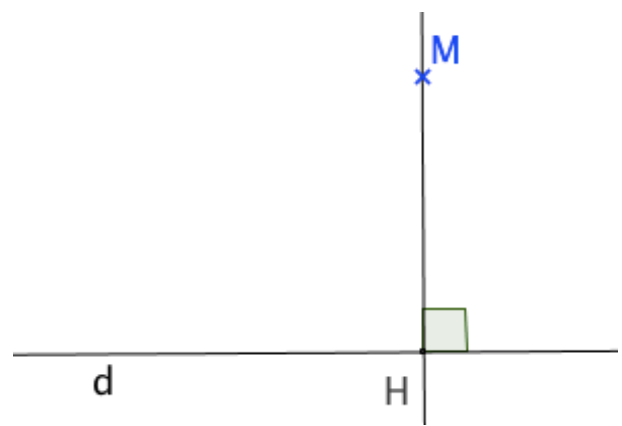
\includegraphics[width=0.8\textwidth]{proj.png}
\end{minipage}%

\end{mdframed}

\begin{mdframed}[
    linewidth=1pt,
    roundcorner=5pt,
    linecolor=Red,
    innertopmargin=10pt,
    innerbottommargin=10pt
]
{\color{red}
\textbf{\underline{Propriété :}}

\vspace{5pt}
Le projeté orthogonal du point $M$ sur la droite $(d)$ est le point de la droite $(d)$
 le plus
proche du point $M$.
}
\end{mdframed}

\newpage
\begin{mdframed}[
    linewidth=1pt,
    roundcorner=5pt,
    linecolor=RoyalBlue,
    innertopmargin=10pt,
    innerbottommargin=10pt
]
{\color{RoyalBlue}
\textbf{\underline{Exercice d'application n°8:} Reconnaitre et construire un projeté 
orthogonal.}}

\begin{minipage}[t]{.45\textwidth}%
    \vspace{0pt}
    1) Donner le projeté orthogonal de :

    \hspace{1cm}a) $C$ sur $(AB)$ \hspace{1cm}b) B sur $(DF)$

    \hspace{1cm}c) $D$ sur $(AC)$ \hspace{1cm}d) F sur $(AD)$

    \vspace{10pt}
    2) Représenter sur la figure le projeté
    orthogonal de :

    \hspace{1cm}a) $C$ sur $(BF)$. Nommer ce point $M$.

    \hspace{1cm}b) $F$ sur $(AB)$. Nommer ce point $N$.
\end{minipage}%
\hfill
\begin{minipage}[t]{.5\textwidth}%
    \vspace{-10pt}
    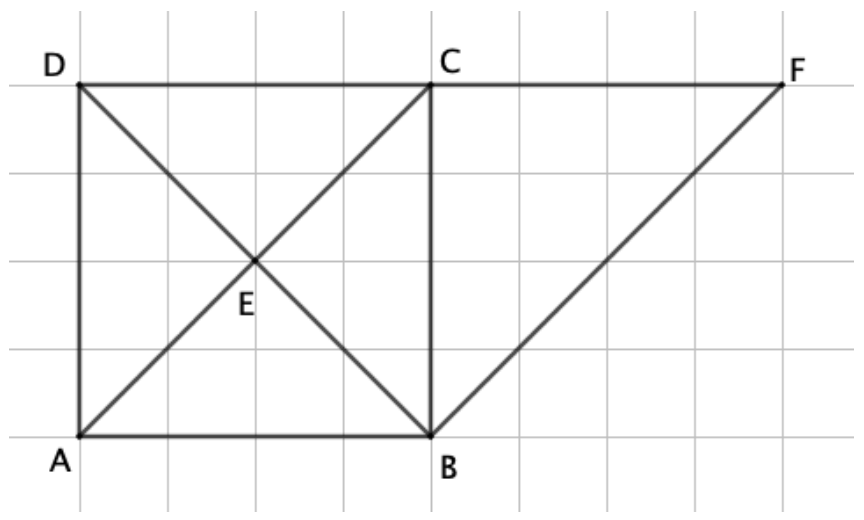
\includegraphics[width=1\textwidth]{exo8.png}
\end{minipage}%

\vspace{0.5cm}
{\color{black!30}\dotfill}

\vspace{0.5cm}
{\color{black!30}\dotfill}

\vspace{0.5cm}
{\color{black!30}\dotfill}

\vspace{20pt}


\end{mdframed}


\end{document}
